%\chapter{Vorlesung}
\begin{figure}[h]
\centering
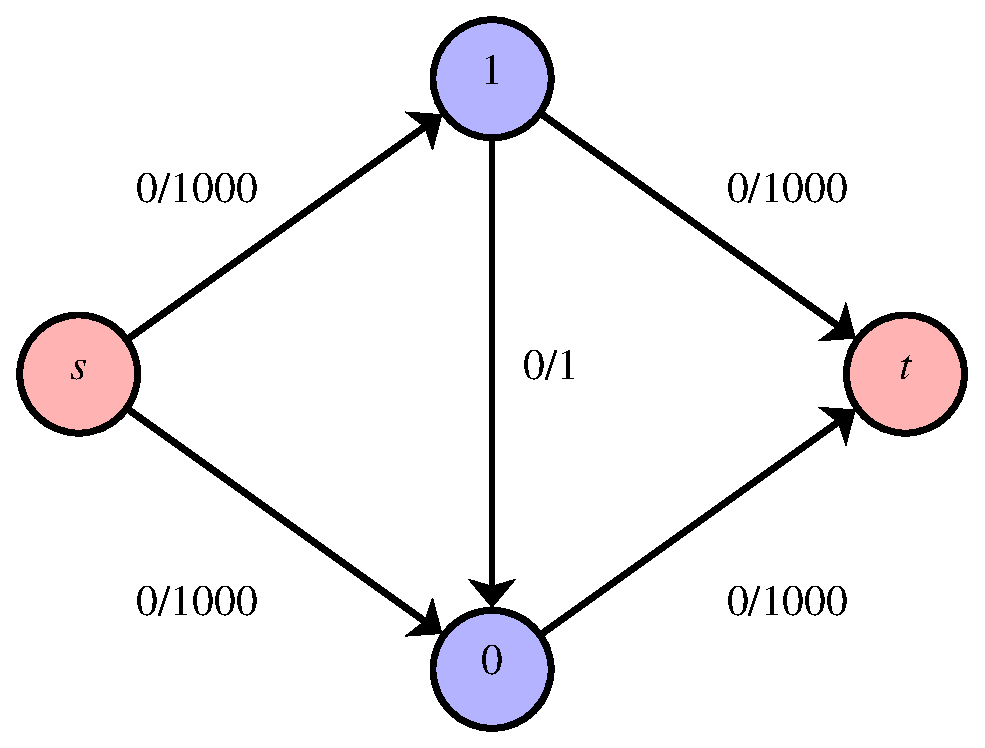
\includegraphics[width=0.4\linewidth]{26/Grafik/Diagramm1}
\caption{Wiederholung}
\label{fig:Diagramm1}
\end{figure}

%Grafik 1 zur Wiederholung
\section{Edmonds-Karp Algorithmus}
\[ G=(V,E)~~,c:R\rightarrow\mathbb{R}^+_0,G_F=(V,E_f), G^L_f=(V,E^L_f) \]
\begin{lstlisting}[style = pseudo]
f = 0;
while($\exists~p \rightsquigarrow t\in G^L_f = (V,E^L_f)$) {
	sei $c_{min}$(p) die kleinste Restkapazität auf p
	$f(u,v)=\begin{cases}
	f(u,v)+c_{min}(p)&\text{falls }(u,v)\in p\\
	f(u,v)-c_{min}(p)&\text{falls }(v,u)\in p
	\end{cases}$
} 
\end{lstlisting}
$\delta_f(s,v)$ die kleinste Zahl von Kanten, die in $G^L_f$ benötigt werden, um von $s$ nach $v$ zu gelangen.
\subsection{Lemma:}
Im Verlauf des Edmonds-Karp Algorithmus gilt:
\[ \delta_{f'}(s,v) \geq \delta_f(s,v) \]
wobei der Fluss $f'$ durch eine Flussverbesserung aus $f$ hervorgegangen ist.
\subsection{Beweis durch Widerspruch}
\subsubsection{Annamhe}
\[ \exists v\in V:\delta_{f'}(s,v)<\delta_f(s,v) ~~~~~(**)\]
sei $v$ so gewählt, dass $\delta_{f'}(s,v)$ minimal.\\
Sei $s\rightsquigarrow u\rightarrow v$ ein kürzester Weg in $G^L_{f'}$.
\[ \delta_f(s,u)\leq\delta_{f'}(s,u) = \delta_{f'}(s,v)-1~~~~~(*) \]
\subsubsection{Behauptung}
\[ (u,v) \notin E^L_f \]
\paragraph{Beweis} durch Widerspruch
\subparagraph{Annahme} $(u,v)\in E^L_f$\\
\[ \delta_f(s,v)\leq\footnote{Dreiecksungleichung}\delta_f(s,u)+1\leq\footnote{wegen $(*)$}\delta_{f'}(s,v) ~~\lightning\text{ zu }(**) \]
\begin{align*}
\hline
\end{align*}
\[ \Rightarrow (u,v)\notin E^L_f\text{ aber } (u,v)\in E^L_{f'} \]
\begin{figure}[h]
\centering
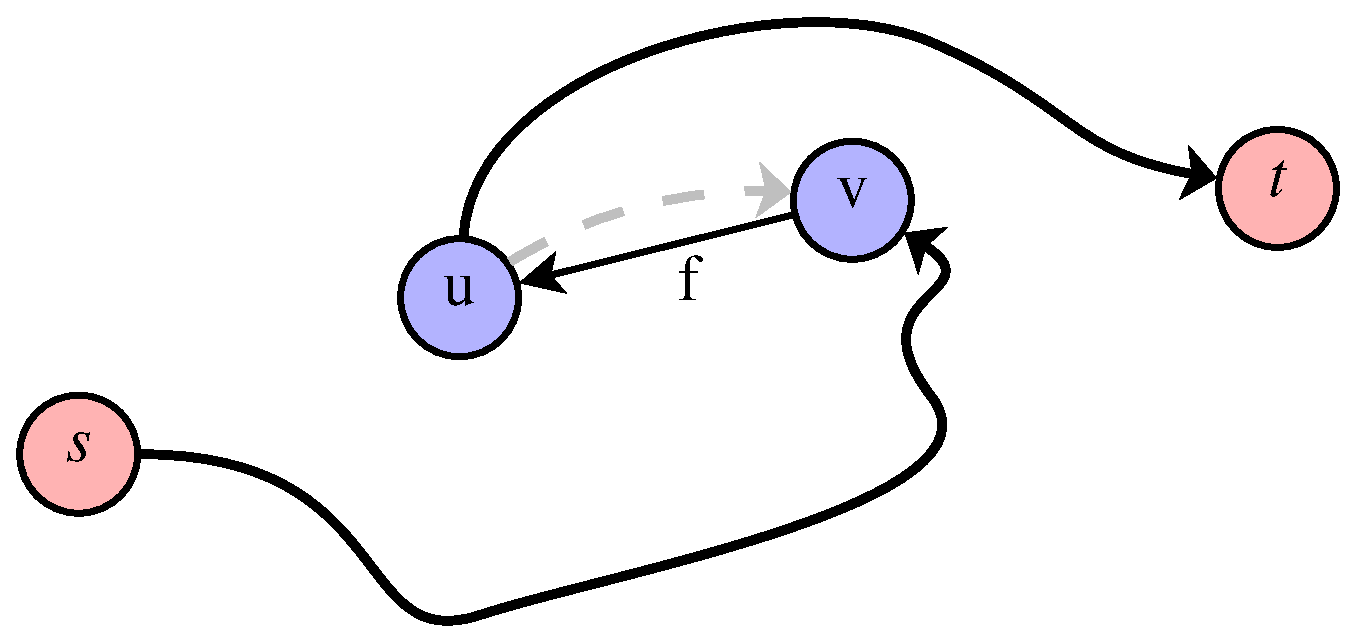
\includegraphics[width=0.4\linewidth]{26/Grafik/Diagramm2}
\caption{}
\label{fig:Diagramm2}
\end{figure}

%Grafik 2
d.h. Bei der Flussverbesserung von $f$ zu $f'$ wurde die Kante $(v,u)$ benutzt in $G^L_{f}$.
\begin{align*}
\delta_f(s,u)&=\delta_f(s,v)+1\\
 &\overset{(**)}{>}\delta_{f'}(s,v)+1\\
 &\overset{(*)}{\geq}\delta_f(s,u)+2 \lightning
\end{align*}
\begin{flushleft}
	q.e.d.
\end{flushleft}
\subsection{Lemma}
Eine kante $(u,v)$ kann un den Level-Rest-Netzwerken höchstens $\frac{|V|}{2}$ mal saturiert werden und damit temporär aus dem jeweiligen Rest-Netzwerk verschwinden
\subsection{Beweis}
\begin{figure}[h]
\centering
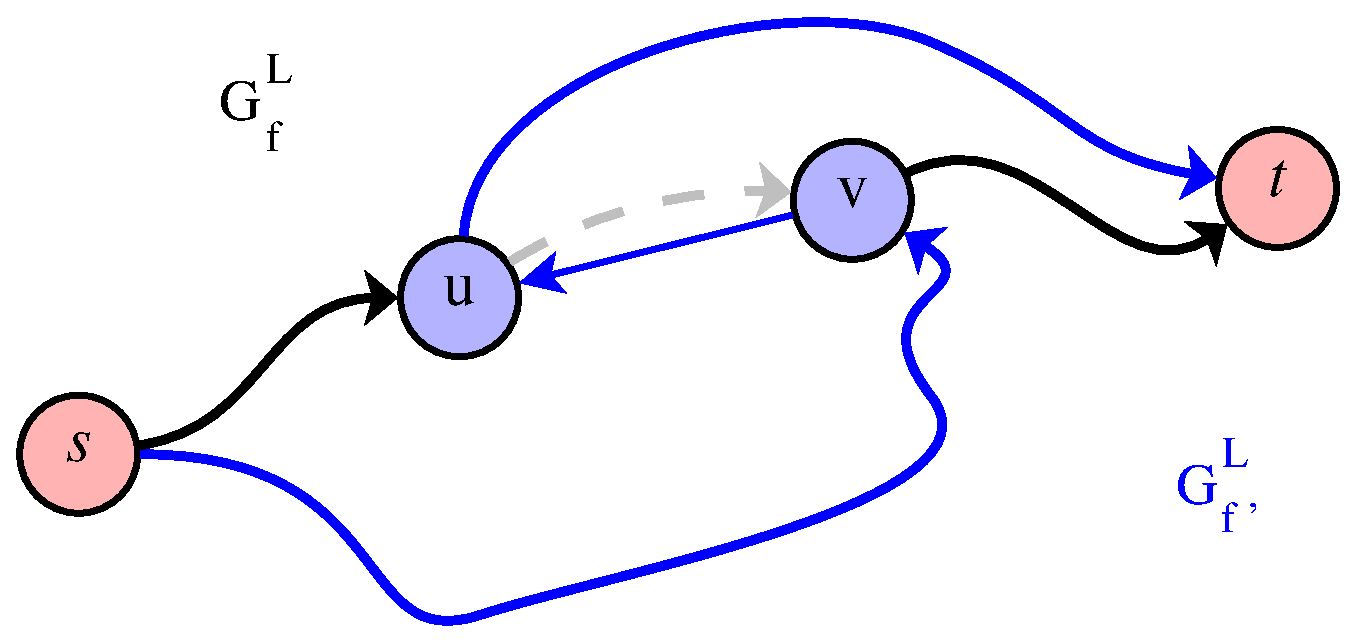
\includegraphics[width=0.4\linewidth]{26/Grafik/Diagramm3}
\caption{}
\label{fig:Diagramm3}
\end{figure}

%Grafik 3
\[ \delta_f(s,v) = \delta_f(s,u)+1 \]
\[ \delta_{f'}(s,v)=\delta_{f'}(s,u)-1 \]
%\begin{align*}
%\hline
%\end{align*}
\[ \delta_f(s,u)=\delta_f(s,v)-1 \leq \delta_{f'}(s,v)-1=\delta_{f'}(s,u)-2 \]
\[ \Rightarrow \delta_{f'}(s,u)\geq \delta_f(s,u)+2 \]
\begin{flushright}
	q.e.d.
\end{flushright}
\subsection{Laufzeitanalyse von Edmonds-Karp Algorithmus}
Bei jeder Flussverbesserung wird mindestens eine Kante saturiert. Jede einzelne Kante kann aber höchstens $\frac{|V|}{2}$ mal saturiert werden.\\
$\Rightarrow$ Es gibt höchstens $\mathcal{O}(|E|\cdot|V|)$ viele Flussverbesserungen, Jede Flussverbesserung kann in $\mathcal{O}(|E|)$ ausgeführt werden.\\
$\Rightarrow$ Gesamtlaufzeit: $\mathcal{O}(|E|^2\cdot|V|)$
\section{Algorithmus von Dinic}
\subsection{Sperrfluss (blocking flow)}
\[ G^L_f=(V,E^L_f) \]
Wir konstruieren einen Sperrfluss $g$ für einen Graphen $H$, indem wir wiederholt entlang von $(s,t)$-Pfaden Fluss von $s$ nach $t$ transportieren.\\
Bevor wir diesen Prozess wiederholen, löschen wir saturierte Kanten aus $H$. Läuft man bei der Wegesuche in eine Sackgasse, so muss diese aus $H$ entfernt werden, damit man zu einem späteren Zeitpunkt nicht wieder in diese Sackgasse gerät.
\paragraph{Ziel}
Algorithmus zur Sperrflussberechnung in Zeit $\mathcal{O}(|V|\cdot|E|)$